\subsection{Opis podatkov ter omejitev naloge}

V nalogi smo morali najprej na nek pameten način definirati množico največ 100
tokov; t.j. terk $\left(\textrm{začetni kot}, \textrm{končni kot}, \textrm{kvaliteta}\right)$. Nato je bilo potrebno za
vsako (približno) desetinko sekunde za 4 sekunde vnaprej napovedati, katere
izmed vnaprej pripravljenih tokov je potrebno uporabniku naložiti v
predpomnilnik za zagotavljanje čim večje kvalitete videa znotraj uporabnikovega
zornega kota. Ta je obsegal vsega skupaj $61$ stopinj, torej po $30$ stopinj na
vsako stran od njegovega trenutnega pogleda. V ta namen smo dobili prejšnje 4
sekunde uporabnikovega dejanskega pogleda.

Poleg tega sta tu veljali še dve dodatni omejitvi: pasovna širina vseh
prenesenih tokov v vsakem trenutku ne sme presegati vrednosti $10000$, za
vsakega ot $360$ kotov pa moramo zagotoviti vsaj kvaliteto $1\%$.

Podani učni podatki so obsegali 86 t.i. sledi (množic terk (čas, kot
uporabnika)), kjer je bila časovna resolucija podana na približno $1/10$
sekunde, kotna resolucija pa na $2$ stopinji natančnosti. 

Za testne podatke smo nato prejeli še 728 sledi po 8 sekund, pri čemer smo za
prve 4 sekunde dobili podan eksakten kot uporabnika, naslednje 4 pa smo morali
napovedati.

Pred začetkom snovanja algoritma se seveda izplača pregledati podatke. Graf
\ref{fig:rel} predstavlja relativne premike uporabnikov v kotih na desetinko sekunde.
Iz tega grafa lahko razberemo, da največkrat uporabniki ne premikajo svoje
glave, ali pa pogled premikajo relativno počasi. Razlog, da sta na histogramu
stolpca $1\degree$ in $-1\degree$ tako nizka leži v tem, da je premik v
podatkih podan na $2$ stopinji natančno.

\begin{figure}[H]
  \centering
  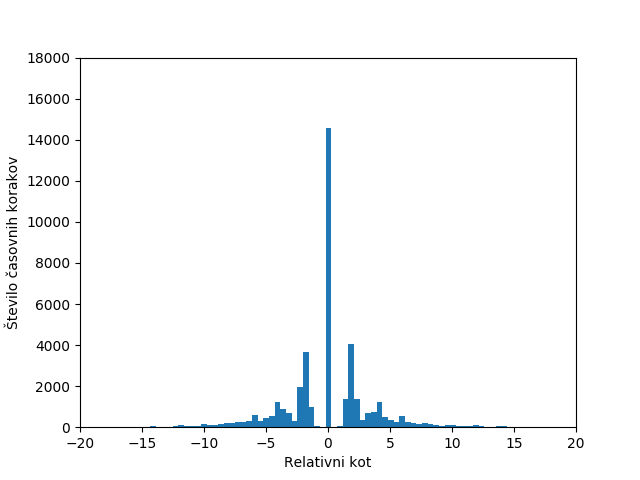
\includegraphics[width=230pt]{{img/rel_moves}}
  \caption{Histogram relativnih premikov v učni množici.}
  \label{fig:rel}
\end{figure}

Grafi \ref{fig:heatmap} prikazujejo vročinske slike \eng{heat map} pogledov
uporabnikov iz učne množice. Pri tem so bile različne slike ustvarjene tako, da
smo označili vseh $61\degree$, ki jih uporabniku prikažemo, ter kote spustili
skozi okna. To lahko razložimo s tem, da v nekem trenutku uporabnika ne zanima
le popolna sredina njegovega pogleda, temveč so pomembni tudi preostali koti,
to pomembnost pa lahko določimo z različnimi okni; npr. Kronecker-delta okno
predpostavi, da je pomembna zgolj sredina pogleda, pravokotno okno predvideva
da je enako pomemben cel pogled, medtem ko Welch okno dodeli večjo pomembnost
sredini pogleda in vedno manjšo pomembnost z oddaljenostjo od sredine.

\begin{figure}[H]
  \centering
  \begin{subfigure}{0.33\textwidth}
    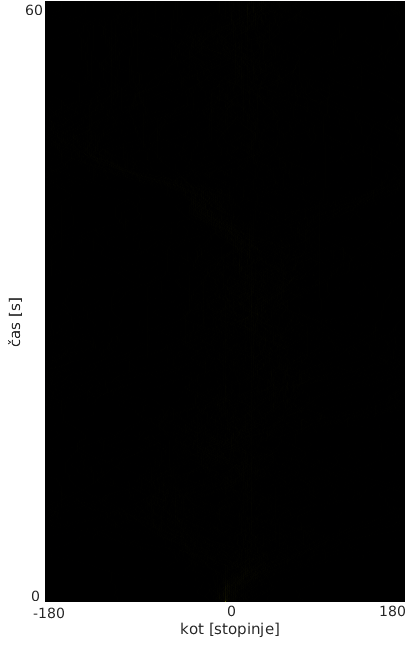
\includegraphics[width=\textwidth]{{img/mp_kr}}
  \end{subfigure}~
  \begin{subfigure}{0.33\textwidth}
    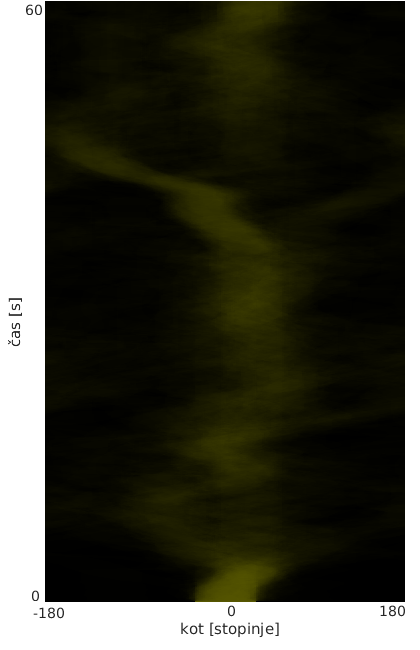
\includegraphics[width=\textwidth]{{img/mp_re}}
  \end{subfigure}~
  \begin{subfigure}{0.33\textwidth}
    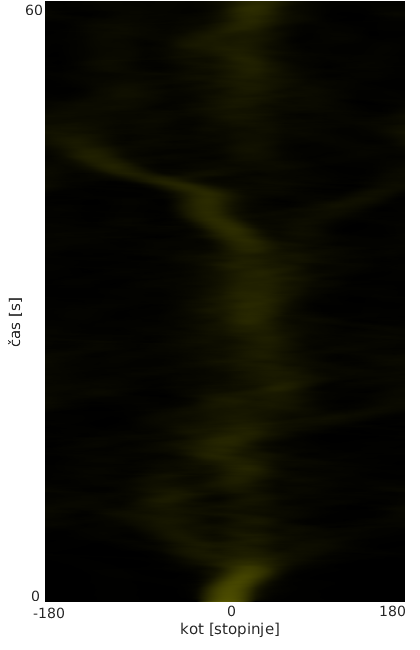
\includegraphics[width=\textwidth]{{img/mp_we}}
  \end{subfigure}
  \begin{subfigure}{0.33\textwidth}
    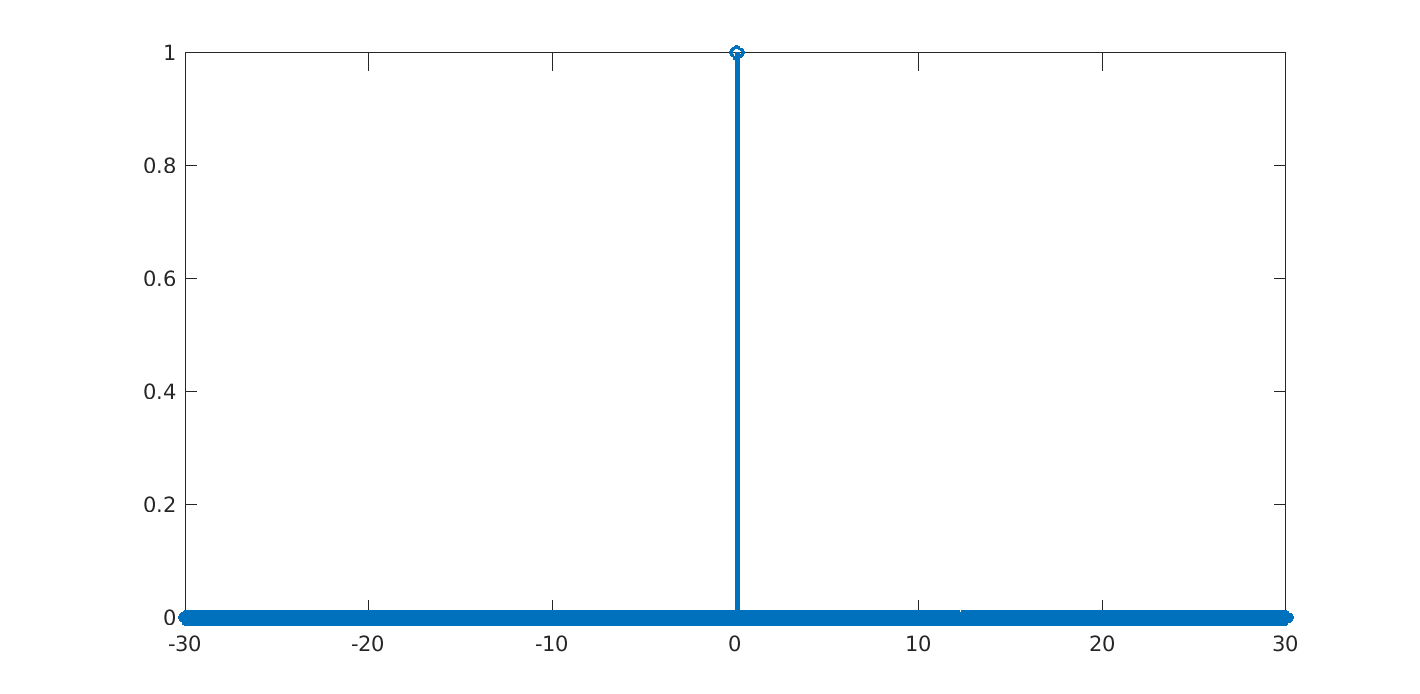
\includegraphics[width=\textwidth]{{img/win_kr}}
  \end{subfigure}~
  \begin{subfigure}{0.33\textwidth}
    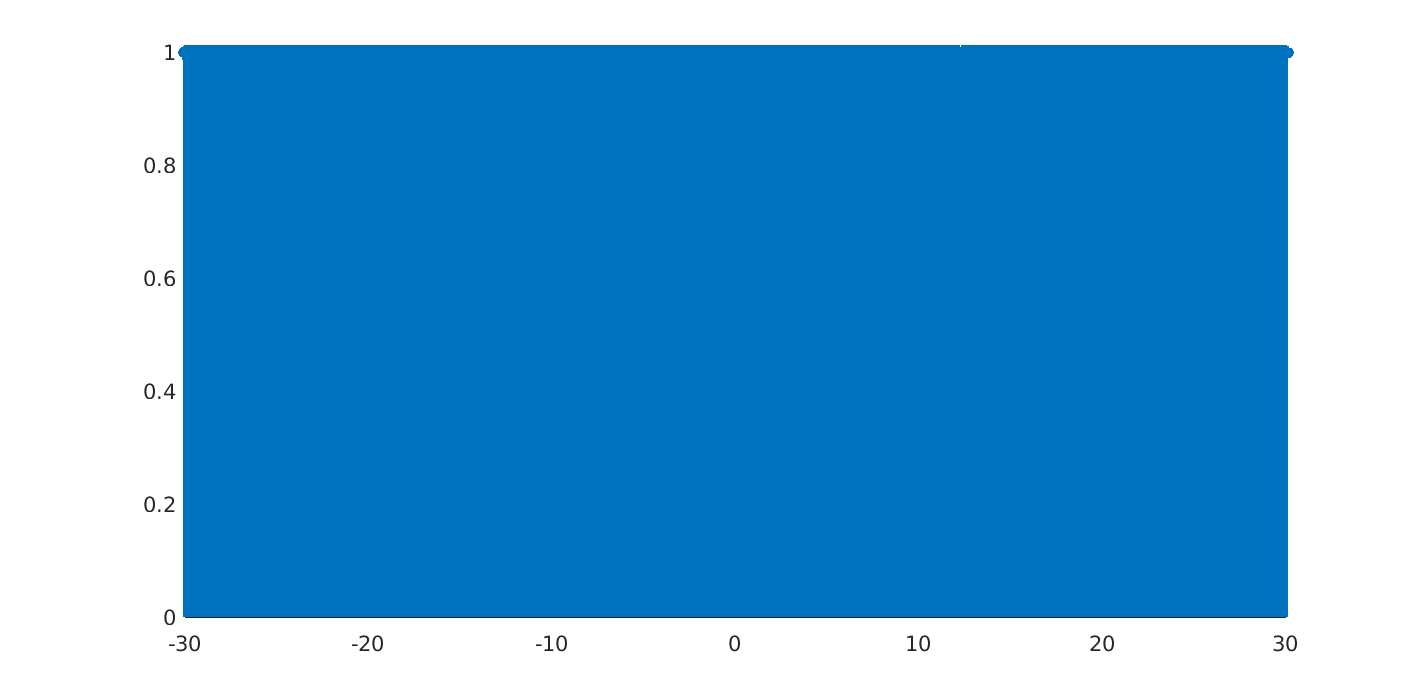
\includegraphics[width=\textwidth]{{img/win_re}}
  \end{subfigure}~
  \begin{subfigure}{0.33\textwidth}
    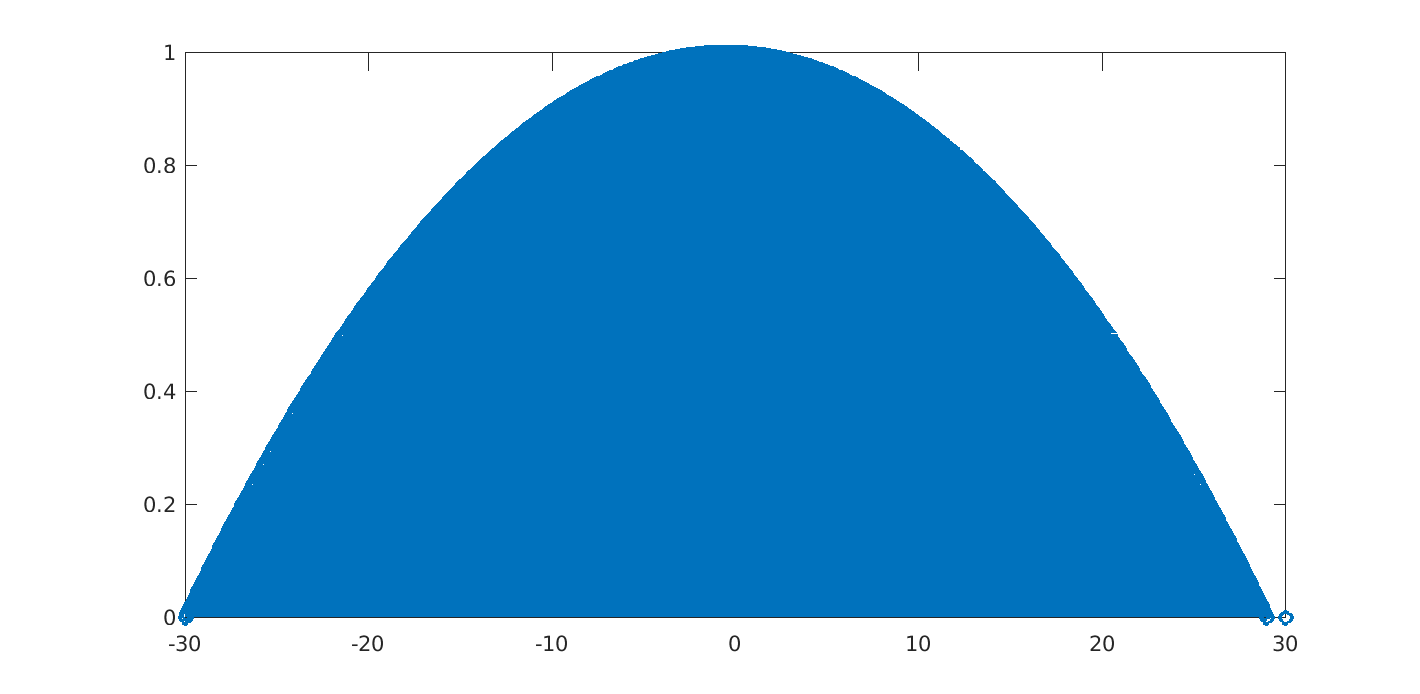
\includegraphics[width=\textwidth]{{img/win_we}}
  \end{subfigure}
  \caption{Vročinske slike izdelane z različnimi okni nad učno množico. Bolj
  rumena barva pomeni večjo vrednost. V zgornji vrstici od leve proti desni:
  izdelane s Kroneckerjevim oknom, s pravokotnim oknom in s Welchovim oknom.
  Pod njimi slike pripadajočih oken.}
  \label{fig:heatmap}
\end{figure}
